\begin{figure*}[t]
\centering
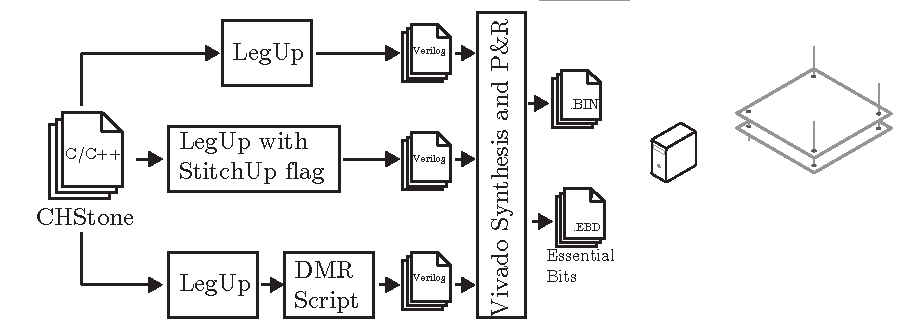
\includegraphics[width=6in]{./imgs/ExperimentFlow.pdf}
\caption{The experiment flow}
\label{fig:ExperimentFlow}
\end{figure*}

To test the error mitigation abilities of StitchUp generated circuits we have adopting the
gold standard of hardware fault injection, where configuration bits on the 
FPGA device are flipped from their original state.
Typical FPGA designs will require a large number of configuration bits often making
full exhaustive testing infeasible, and usually results in the adoption of random
testing. 
However in our case we have developed an experiment
platform allowing us to achieve full exhaustive fault injection in reasonable time
and where possible we have used this to test StitchUp on the popular CHStone 
HLS benchmarks.

We make use of many low cost Xilinx FPGA SoC devices known as
Zedboards all injecting on the same circuit in parallel.
Each Zedboard runs a full Linux OS on its hardened ARM processor and is arranged into
a cluster managed by a single desktop\footnote{called The SoC Drawer}.

In each FPGA circuit a Xilinx Soft Error Mitigation (SEM) IP Core 
connected to the FPGA internal configuration port (ICAP) is responsible for 
flipping configuration bits.
This approach was made possible due to the latest release of LegUp
(v4.0) supporting the generation of generic Verilog circuits, enabling it to be compiled
to Xilinx devices.
Both the SEM core and the StitchUp circuitwas instantiated and connected to the 
ARM processing system via AXI interconnects.  
Software running under Linux on each of the ARM cores was then responsible for, sending the
address and injection command to the SEM core, starting the circuit under test, and
collecting the result from that circuit. 

Figure \ref{fig:ExperimentFlow} shows an overview of the experiment setup.
Each circuit at the top is fed into three different flows:
On the  left a full DMR version of the circuit is built which uses LegUp to generate a 
single circuit, instantiated it twice, and 
generate comparison logic on the state register and output value;
in the middle a circuit, generated using the StitchUp flow protecting only the control
structure of the original circuit; and on the right the original circuit with no protection
is produced via a standard LegUp pass.

Each different version is then passed through the Xilinx FPGA circuit tool flows to produce
two files, an essential bits file (.EBD), and a configuration binary (.BIN).
The essential bits file is a list of configuration memory bits that have any
influence on our generated circuit, and is used to reduce the number of injections
required to fully test our design\footnote{essential bits do not contain BRAM data, since these are considered transient data not essential}.

Both the EBD and BIN files are then sent to The SoC Drawer where they are allocated to
devices for testing, if they are small enough then they are allocated to run on the 
cluster of Zedboards where they will be exhaustively tested, while the larger circuits 
are allocated to a larger ZC706 device for random testing.
Designs allocated to the Zedboards have their EBD files divided up
into smaller chunks and each chunk is processed in parallel on a different Zedboard device.

\subsection{Performing the error injection}
Software running on the ARM of each Zedboard performs each indivudal injection experiment
and is responsible for, injecting a fault, 
running the circuit, and storing the result.
The fault is then repaired by re-injecting an error into the
same configuration memory location (i.e. flipping the bit back to it's original state)
and moves onto the next essential bit address.
Some fault may cause the circuit to never terminate so if no response is seen within three orders
of magnitude of it's expected time a timeout halts its execution and keeps a record of it.

The results are then analysed and each outcome is classified into three separate categories:

\begin{enumerate}
\setlength{\itemsep}{1pt}
\setlength{\parskip}{0pt}
\setlength{\parsep}{0pt}
\item Execution Time Error - This is where the execution of the circuit either took
an incorrect number of cycles to complete or timed out. Errors of these type are
control flow related since any deviation from the correct execution path will cause
an incorrect number of cycles.
\item Data-Flow Only Errors - These are errors where the circuit has returned an incorrect
data result but has executed in the correct number of cycles, such as error caused
by faults in a non-control structure functional unit.
\item Caught Errors - These are errors that were detected by the protection method, which is
either DMR or StitchUp.
\end{enumerate}
